% @Author: Sol W Courtney
% @Date:   2018-03-18 23:08:02
% @Last Modified by:   Sol W. Courtney
% @Last Modified time: 2018-03-19 00:38:14
\documentclass[11pt,a4paper,fleqn,notitlepage,oneside]{article}
\input{01_UsePackages}
\input{02_Settings}
\input{03_Title}
\begin{document}
\maketitle
\input{04_Abstract}
\input{05_MainImage}

\input{10_BasicIdea}
\input{20_Computation}
\input{30_GeneralProps}
\input{40_Accuracy}




\section{Numbers and Maximums} % (fold)
	\label{sec:numbers}
	Features as a function of radial displacement.
	We loose stars per unit area with radius but we gain contrast and numbers of features.

	\begin{figure}[H]
		\includegraphics[width=17cm]{23_n_features.png}
		\caption{
			Here we see the total number of registered features as a function of radius.
			Each BJ halo was used once for this plot.
			11 halos total.
		}
		\label{fig:n_features}
	\end{figure}
	%
	\begin{figure}[H]
		\includegraphics[width=17cm]{10_xbox_max.png}
		\caption{
			Here we see the maximum contrast density value as a function of radius.
			The y axis value represents how many times more stars are in the feature compared with the average number of stars per box plus or minus 1 percent radius. 
		}
		\label{fig:xbox_max}
	\end{figure}

	\begin{figure}[H]
		\includegraphics[width=17cm]{24_log10(xbox_max).png}
		\caption{
			Here we see the Log10 maximum contrast density value as above. 
		}
		\label{fig:24_log10(xbox_max)}
	\end{figure}

	\begin{figure}[H]
		\includegraphics[width=17cm]{20_Log10(n_stars).png}
		\caption{
			Here we see the log10 value of the number of stars within each feature as a function of radius. 
		}
		\label{fig:n_stars}
	\end{figure}

% section numbers (end)


\section{Summary} % (fold)
	\label{sec:summary}


	\begin{figure}[H]
		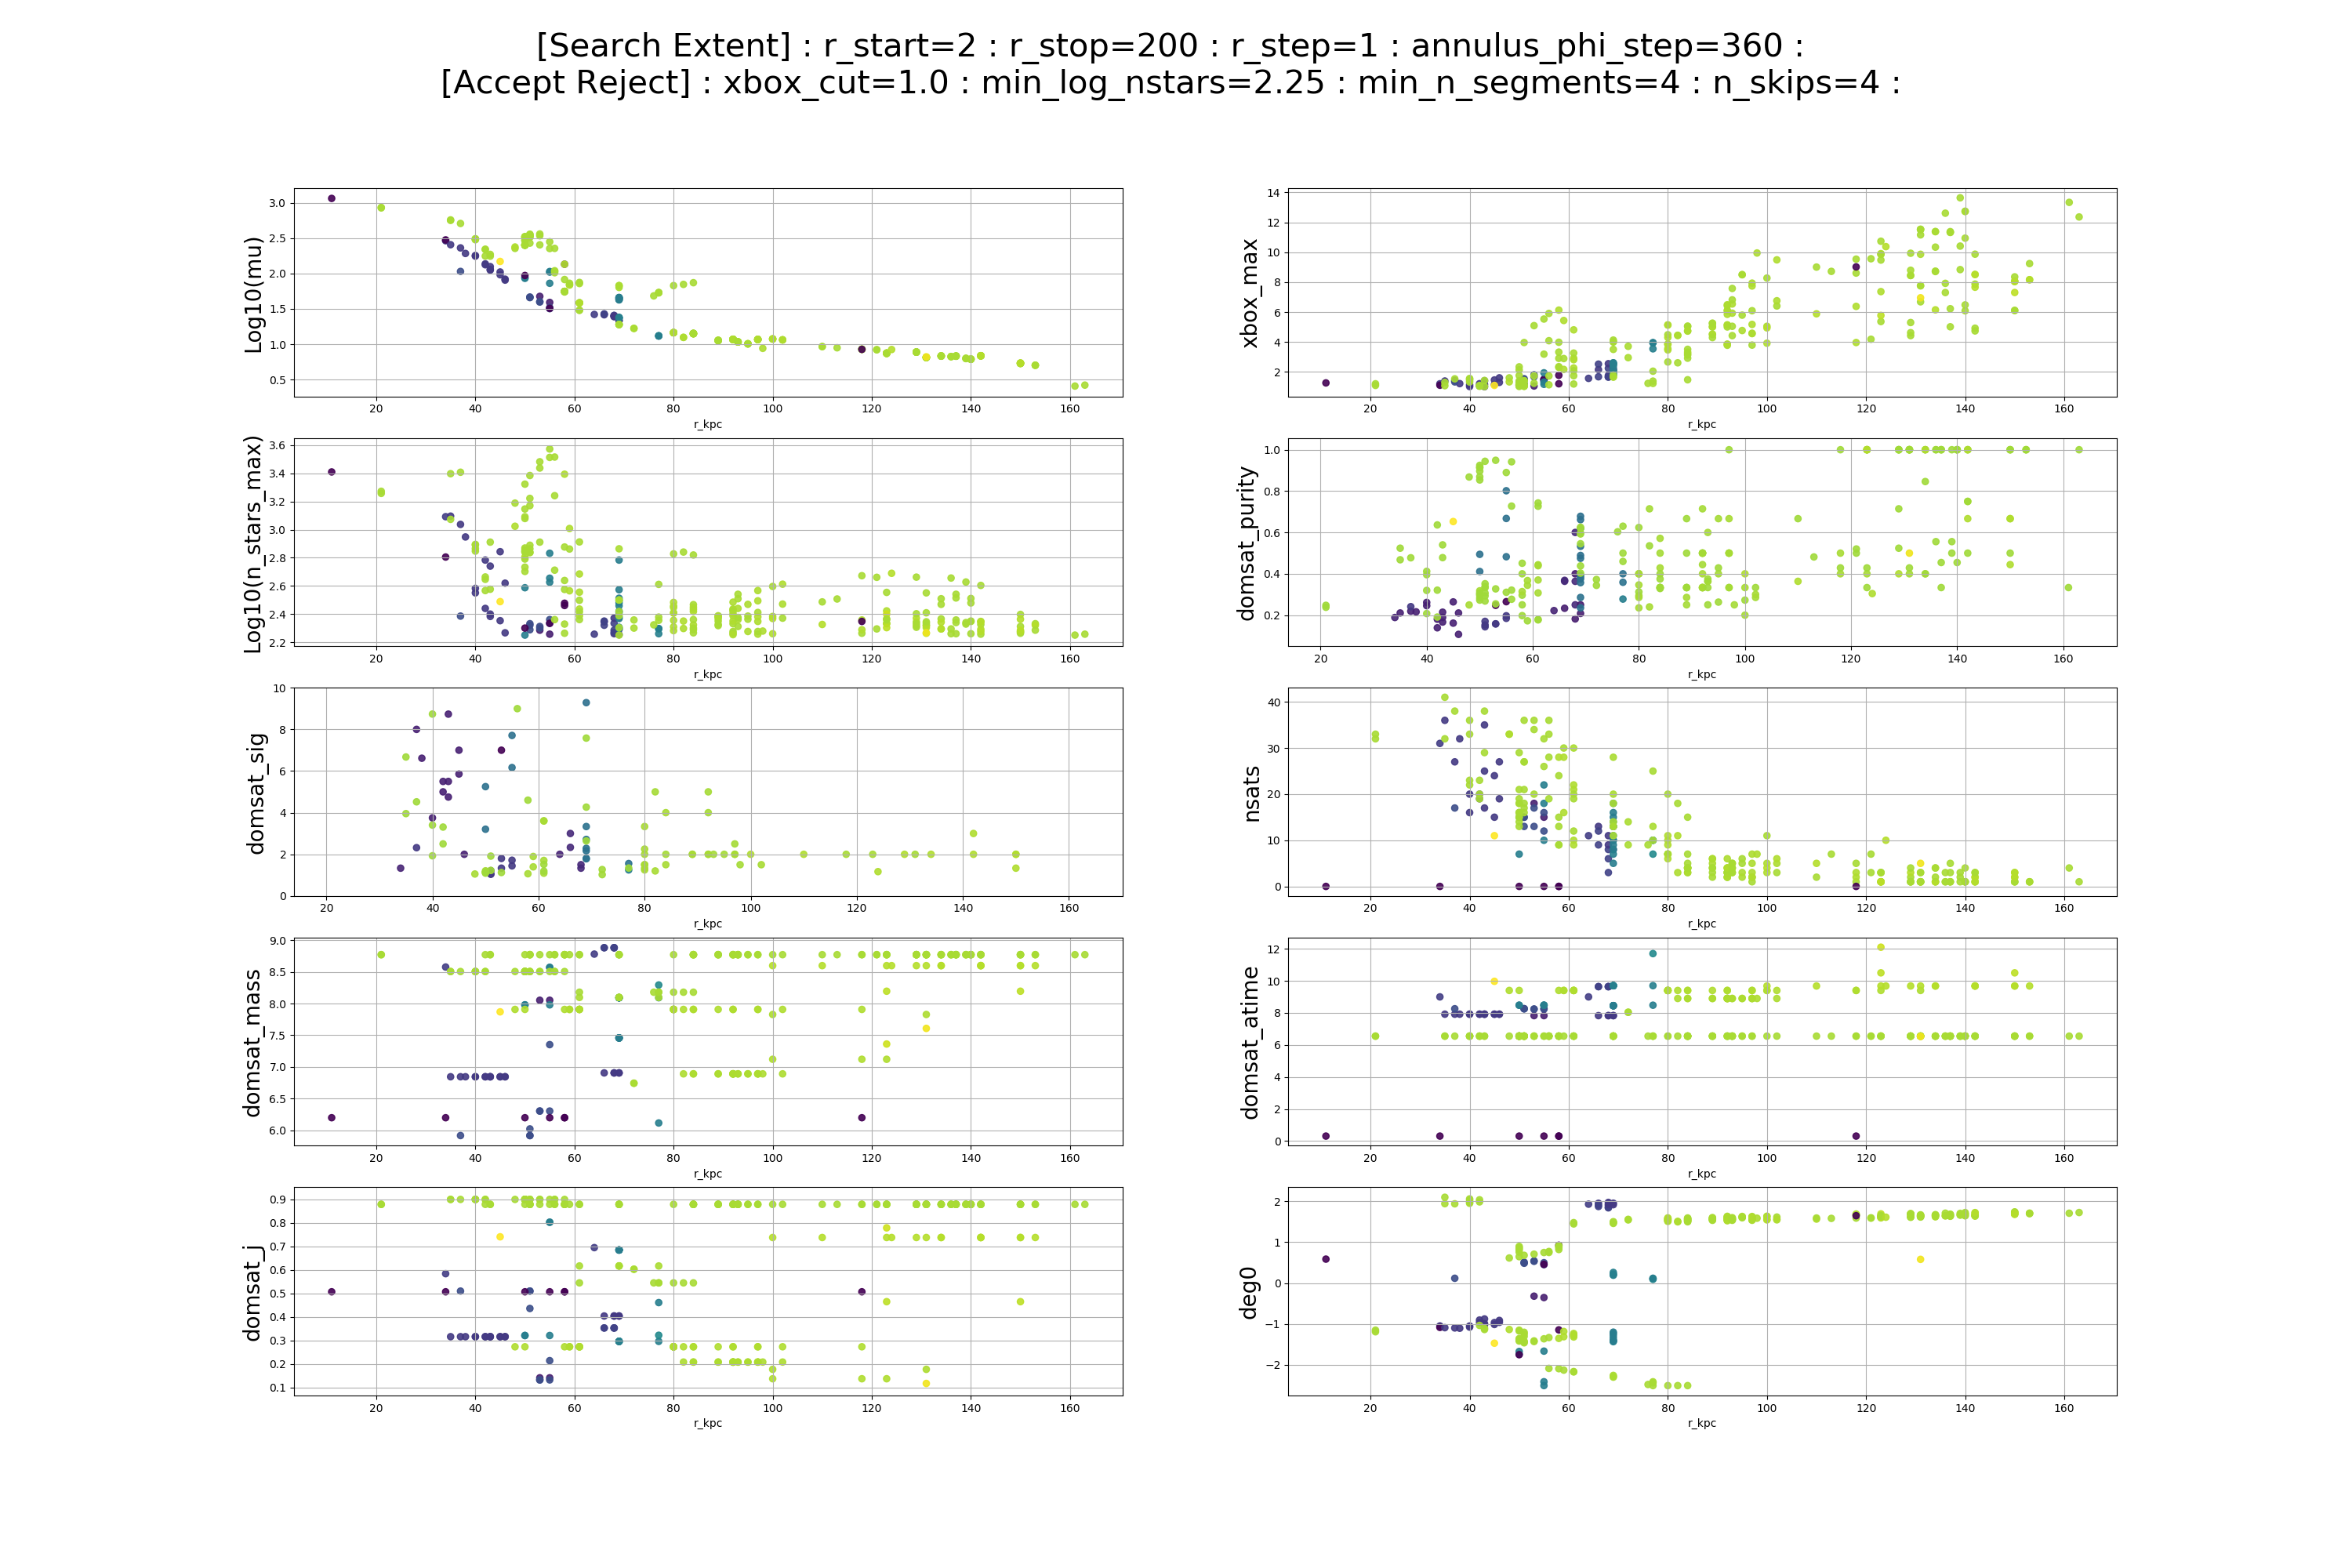
\includegraphics[width=17cm]{all_halo_summary_plot.png}
		\caption{
			Summary plot of all halos colored to halo number. 
		}
		\label{fig:all halos - summary plot}
	\end{figure}

% section summary (end)


\section{Interesting Plot Action} % (fold)
	\label{sec:interesting_plot_action}

	\begin{figure}[H]
		\includegraphics[width=17cm]{Log10(mu)_vs_Log10(n_stars)_0.png}
		\caption{
			is this good? 
		}
		\label{fig:Log10(mu)_vs_domsat_purity_5}
		\end{figure}

	\begin{figure}[H]
		\includegraphics[width=17cm]{Log10(mu)_vs_domsat_atime_1.png}
		\caption{
			? 
		}
		\label{fig:Log10(mu)_vs_domsat_purity_5}
	\end{figure}

	\begin{figure}[H]
		\includegraphics[width=17cm]{Log10(mu)_vs_domsat_purity_4.png}
		\caption{
			? 
		}
		\label{fig:Log10(mu)_vs_domsat_purity_5t}
	\end{figure}

	\begin{figure}[H]
		\includegraphics[width=17cm]{extent_vs_Log10(n_stars)_27}
		\caption{
			? 
		}
		\label{fig:extent_vs_Log10(n_stars)_27}
	\end{figure}
% section interesting_plot_action (end)

\end{document}


